\documentclass{report}
\usepackage{amsmath, amssymb, amsthm}
\usepackage{geometry}
\geometry{a4paper, margin=0.8in}
\usepackage{float}
\usepackage{graphicx} % ADDED FOR IMAGES
\usepackage{tikz}
\usetikzlibrary{calc, decorations.pathreplacing}
\usepackage{pgfplots}
\pgfplotsset{compat=1.18}
\usepackage{xcolor}
\usepackage{tcolorbox}
\tcbuselibrary{theorems}
\usepackage{eurosym}
\usepackage{fancyhdr}
\usepackage{booktabs}
\usepackage{listings}

\lstdefinestyle{tcblatex}{
    language=[Visual]Basic,
    basicstyle=\ttfamily\footnotesize,
    keywordstyle=\bfseries,
    commentstyle=\itshape,
    stringstyle=\ttfamily,
    showstringspaces=false,
    breaklines=true,
    columns=fullflexible
}

\begin{document}

\pagestyle{fancy}
\fancyhf{}
\rhead{Report 5 \;|\; Stochastic Methods for Finance \;|\; \thepage}
\renewcommand{\headrulewidth}{0.4pt}
\setlength{\headheight}{14pt}
\thispagestyle{plain} 

% --- PROFESSIONAL HEADER ---
\begin{flushleft}
    {\large \textbf{Stochastic Methods for Finance - Report 5}} \\
    \rule{\textwidth}{0.4pt} \\ 
    \textbf{Author:} Davide Quartucci \hfill \textbf{Date:} April 15, 2026 \\
    \textbf{Asset:} ADYEN NV - ADYEN.AS \\
\end{flushleft}

\begin{center}
    \fcolorbox{black}{gray!10}{
        \begin{minipage}{0.95\textwidth}
            \small \textit{Every step implementation can be checked in the provided file:} \texttt{Report5\_Quartucci\_Davide.xlsm}
        \end{minipage}
    }
\end{center}

\section{Setup and Parameters}
 
The Black--Scholes (B\&S) model is used for pricing vanilla European options.
The reference parameters are:
\[
  K = 100, \qquad r = 1\%, \qquad \sigma_{\mathrm{base}} = 20\%.
\]
The state-variable grid is:
\[
  S \in \{60, 65, 70, \ldots, 130, 135, 140\}, \qquad
      \tau \in \{0.1, 0.2, 0.3, 0.4, 0.5, 0.6, 0.7, 0.8, 0.9, 1, 2, 3, 4, 5\}\ \text{years}.
\]
 
\subsection{Review of B\&S formulas and Greeks}
 
Under the standard assumptions of the B\&S model, the
price of a European \emph{call} is:
\[
  C = S\,\Phi(d_1) - K e^{-r\tau}\,\Phi(d_2),
\]
and the price of a European \emph{put}, via put-call parity, is:
\[
  P = K e^{-r\tau}\,\Phi(-d_2) - S\,\Phi(-d_1),
\]
where
\[
  d_1 = \frac{\ln(S/K) + (r + \tfrac{1}{2}\sigma^2)\tau}{\sigma\sqrt{\tau}},
  \qquad
  d_2 = d_1 - \sigma\sqrt{\tau},
\]
and $\Phi(\cdot)$ is the cumulative distribution function of the standard normal.
 
The B\&S Greeks for the call are:
\begin{align*}
  \Delta_C = \Phi(d_1) \quad\, \Gamma = \frac{\phi(d_1)}{S\,\sigma\sqrt{\tau}} \quad\,\,
  \Theta_C = -\frac{S\,\phi(d_1)\,\sigma}{2\sqrt{\tau}}
              - r\,K e^{-r\tau}\,\Phi(d_2) \quad\,\,
  \mathcal{V} = S\,\phi(d_1)\,\sqrt{\tau} \quad\,\,
  \rho_C   = K\,\tau\,e^{-r\tau}\,\Phi(d_2)
\end{align*}
where $\phi(\cdot) = \Phi'(\cdot)$ is the standard normal density.
For the put, the symmetry relations implied by put-call parity give:
\[
  \Delta_P = \Delta_C - 1, \qquad
  \Gamma_P = \Gamma_C, \qquad
  \mathcal{V}_P = \mathcal{V}_C, \qquad
  \Theta_P = \Theta_C + r K e^{-r\tau}, \qquad
  \rho_P = -K\tau e^{-r\tau}\,\Phi(-d_2).
\]
 
\subsection{VBA Script for Computing the Greeks}
 
An Excel VBA script has been implemented in the attached Excel file that computes the five Greeks ($\Delta$,
$\Gamma$, $\Theta$, $\mathcal{V}$, $\rho$) for the call and put on a $17 \times 14$
grid of $(S, \tau)$ values with volatility $\sigma = 20\%$.
 
The main procedure is structured as follows:
\begin{enumerate}
  \item The market constants ($K$, $r$, $\sigma$) and the $S$ and $\tau$ grids are
        declared using one-dimensional arrays.
  \item For each pair $(S_i, \tau_j)$, $d_1$ and $d_2$ are computed using the
        formulas above, with \texttt{Application.NormSDist} for $\Phi$ and the
        analytical expression $\phi(x) = e^{-x^2/2}/\sqrt{2\pi}$ for the density.
  \item The Greeks are written into dedicated cells in the \texttt{CallGkTable} and
        \texttt{PutGkTable} sheets, organized by Greek (DELTA, GAMMA, THETA, VEGA, RHO
        blocks) and by $\tau$ columns.
\end{enumerate}
 
\subsection{Volatility Shock: $\sigma = 30\%$ and $\sigma = 10\%$}
 
Part 2 requires repeating the analysis with a multiplicative \emph{shock} of
$\pm 50\%$ on the base volatility:
\[
  \sigma^- = 20\% \times (1 - 50\%) = 10\%, \qquad
  \sigma^+ = 20\% \times (1 + 50\%) = 30\%.
\]
The results are reported in adjacent columns within the same \texttt{CallGkTable} and
\texttt{PutGkTable} sheets, under the labels \texttt{vol1 = 0.20}, \texttt{vol2 = 0.30},
\texttt{vol3 = 0.10}.
 
The comparative analysis shows the expected behavior: increasing $\sigma$ widens the
risk-neutral distributions, making OTM options more sensitive (Delta farther from zero
or one), increasing Gamma and Vega, and generally lowering the absolute value of Theta
for ATM options over short horizons.
 
\subsection{3D Surfaces of the Greeks}
 
For each of the five Greeks and for the three volatility levels, three-dimensional
surface plots were generated with axes $S$, $\tau$, and the Greek value, available in
the \texttt{Display PART 1} sheet of the attached Excel file.
The main observations are:
 
\begin{itemize}
  \item \textbf{Delta}: It increases monotonically from 0 (deep OTM, $S \ll K$) to 1
        (deep ITM, $S \gg K$) for the call; the same profile shifted by $-1$ for the
        put. As expiry approaches ($\tau \to 0$), the surface becomes increasingly
        steep around ATM ($S \approx K$).
  \item \textbf{Gamma}: Concentrated around $S = K$; the peak grows as expiry
        approaches (the ``pin risk'' effect). Higher volatility flattens and widens the
        peak.
  \item \textbf{Theta}: Always negative (time-value decay); its magnitude is largest
        near ATM for short maturities.
  \item \textbf{Vega}: Also concentrated around ATM; it increases with $\tau$ (longer
        maturity options are more sensitive to volatility).
  \item \textbf{Rho}: Its magnitude increases with $\tau$ and with the degree of ITM;
        the call has positive Rho, the put negative.
\end{itemize}

% PART 1 IMAGE ADDED HERE
\begin{figure}[H]
    \centering
      
\includegraphics[width=0.8\textwidth]{Picture1.png}
    \caption{Theoretical Greek Surfaces (VBA). The horizontal axis represents the Spot Price ($S$), showing the dynamic evolution of the portfolio as the underlying asset price changes.}
    \label{fig:part1_theoretical}
\end{figure}
 
\subsection{Greeks for the Put}
 
The put surfaces are fully analogous to those of the call thanks to the parity
relations listed in Section 0.1.1. In particular, $\Gamma$ and $\mathcal{V}$ are identical for
call and put with the same parameters, as can be checked by comparing the \texttt{GAMMA}
and \texttt{VEGA} blocks in the \texttt{CallGkTable} and \texttt{PutGkTable} sheets.
The put Delta has the opposite sign (range $[-1, 0]$), Theta is slightly less
negative because of the additional $r K e^{-r\tau}$ term, and Rho is negative.
 
% PUT SURFACES IMAGE ADDED HERE
\begin{figure}[H]
    \centering
      % Replace with the actual name of your Put image
    
\includegraphics[width=0.8\textwidth]{Picture2.png} 
    \caption{Theoretical Greek Surfaces for the Put option (VBA). Consistent with put-call parity, the $\Gamma$ and $\mathcal{V}$ surfaces are identical to the Call, while $\Delta$ is strictly negative (ranging from -1 to 0) and $\rho$ is inverted.}
    \label{fig:part1_theoretical_put}
\end{figure}

% ==============================================================
\section{Part 2: Empirical Analysis: ADYEN NV (ADYEN.AS)}
% ==============================================================
 
\subsection{Asset Selection and Market Data}
 
The stock \textbf{ADYEN NV} (Reuters ticker: \texttt{ADYEN.AS}) was selected, a digital
payments company listed on Euronext Amsterdam, which does not pay ordinary dividends,
thus satisfying the B\&S no-dividend assumption.
 
The data were extracted from \textbf{LSEG Workspace} on
\textbf{11 April 2026}. The market parameters are:
\[
  S_0 = 858.8\ \text{EUR}, \qquad
      r = 2.198\%\ \text{(EUR 3-month OIS rate)}.
\]
The three maturities considered in the European options book are:
\[
      \tau_1 = 0.19\ \text{years (19 Jun 2026)}, \quad
      \tau_2 = 0.44\ \text{years (18 Sep 2026)}, \quad
      \tau_3 = 0.69\ \text{years (18 Dec 2026)}.
\]
 
\subsection{Implied Volatility Surface (Call Prices)}
 
Implied volatility was obtained by inverting the B\&S formula on the market mid prices
of the calls, using a bisection algorithm implemented in VBA.
The surface is tabulated in the \texttt{Empirical PART 2} sheet for strikes from
$K = 520$ to $K = 1200$.
 
\begin{table}[H]
\centering
\caption{Sample of mid implied volatility (Call) — ADYEN.AS, 11-Apr-2026}
\begin{tabular}{cccc}
\toprule
$K$ & $\sigma_{\mathrm{IV}}(\tau_1)$ & $\sigma_{\mathrm{IV}}(\tau_2)$ &
$\sigma_{\mathrm{IV}}(\tau_3)$ \\
\midrule
520  & 73.1\%  & 63.2\%  & 58.2\% \\
760  & 56.9\%  & 54.1\%  & 46.6\% \\
860  & 52.8\%  & 51.4\%  & 50.0\% \\
1000 & 48.6\%  & 48.6\%  & 48.4\% \\
1200 & 53.2\%  & 49.5\%  & 44.0\% \\
\bottomrule
\end{tabular}
\end{table}
 
The 3D surface (strike $\times$ maturity $\times$ IV) is available in the
\texttt{Empirical PART 2} sheet of the attached Excel file.
 
\subsection{Volatility Smile, Skew, and Put-Call Parity}

The volatility smile analysis shows a pronounced \emph{negative skew}: OTM puts (low strikes) exhibit systematically higher implied volatility than OTM calls (high strikes), a classic phenomenon in equity markets driven by asymmetric hedging demand and the financial leverage effect. Furthermore, building the surfaces separately for calls and puts reveals important market dynamics:

\begin{itemize}
    \item \textbf{Short-Term Skew ($\tau_1 = 0.19$):} The skew is very pronounced. $\sigma_{\mathrm{IV}}$ falls from about 73\% at $K=520$ to a minimum of roughly 48\%--52\% around ATM, then rises slightly for deep OTM calls (an ``asymmetric smile''). For OTM strikes, the put IV is slightly higher than the call IV, consistent with demand for downside protection.
    \item \textbf{Term Structure Flattening ($\tau_3 = 0.69$):} As maturity increases, the surface tends to flatten and the two surfaces (Call and Put) converge substantially. The IV spread between the strike extremes shrinks, consistent with the mean-reversion theory of stochastic volatility.
    \item \textbf{Put-Call Parity IV Mismatch:} Small violations of inverse put-call parity in IV are observable. These are attributable to bid-ask spreads and to the non-synchronous prices extracted from LSEG Workspace. Furthermore, pure put-call parity relies on the Spot price ($S$), but real markets price European options based on the Forward price ($F$), which embeds implied funding costs. This structural difference prevents the spot-based IVs of calls and puts from perfectly overlapping.
\end{itemize}

% IMMAGINE CALL VS PUT SKEW (ex Figura 4)
\begin{figure}[H]
    \centering
    
\includegraphics[width=\textwidth]{Picture4.png}
    \caption{Implied Volatility Surfaces for Call and Put options. The side-by-side comparison highlights the negative skew typical of equity markets. Minor vertical discrepancies (IV mismatch) reflect market frictions, bid-ask spreads, and forward-rate dynamics.}
    \label{fig:call_put_skew}
\end{figure}
 
\subsection{Smoothness of the Greeks as $\tau$ Increases}
 
The empirical Greeks were computed by applying the B\&S formula with mid implied
volatility as the input $\sigma$, for each pair $(K, \tau_i)$.
The results are reported in the \texttt{Empirical PART 2} sheet, section
\emph{PART 2.4 - SMOOTHNESS OF GREEKS}.
 
For illustration, the Delta and Gamma values around ATM are reported below:
 
\begin{table}[H]
\centering
\begin{minipage}[t]{0.48\textwidth}
\centering
\caption{Delta (Call) mid — ADYEN.AS}
\begin{tabular}{cccc}
\toprule
$K$ & $\Delta(\tau_1)$ & $\Delta(\tau_2)$ & $\Delta(\tau_3)$ \\
\midrule
840  & 0.590 & 0.605 & 0.618 \\
880  & 0.511 & 0.551 & 0.575 \\
920  & 0.432 & 0.497 & 0.530 \\
960  & 0.357 & 0.446 & 0.487 \\
1000 & 0.278 & 0.390 & 0.445 \\
\bottomrule
\end{tabular}
\end{minipage}
\hfill
\begin{minipage}[t]{0.48\textwidth}
\centering
\caption{Gamma (Call) mid — ADYEN.AS}
\begin{tabular}{cccc}
\toprule
$K$ & $\Gamma(\tau_1)$ & $\Gamma(\tau_2)$ & $\Gamma(\tau_3)$ \\
\midrule
840  & 0.0019 & 0.0013 & 0.0011 \\
880  & 0.0020 & 0.0014 & 0.0011 \\
920  & 0.0020 & 0.0014 & 0.0011 \\
960  & 0.0019 & 0.0014 & 0.0011 \\
1000 & 0.0018 & 0.0014 & 0.0012 \\
\bottomrule
\end{tabular}
\end{minipage}
\end{table}
 
The key observations on smoothness are:
 
\begin{itemize}
  \item \textbf{Delta}: The Delta curve as a function of $K$ becomes progressively
        flatter as $\tau$ increases, because the risk-neutral distribution widens. For
        very short $\tau_1$, Delta is almost binary (0 or 1) for options far from ATM.
  \item \textbf{Gamma}: It decreases as $\tau$ increases for ATM options (the peak
        lowers and widens), reducing dynamic delta-hedging risk.
  \item \textbf{Theta}: The absolute time decay tends to decrease for longer maturities,
        but remains negative for long positions.
  \item \textbf{Vega}: It increases with $\tau$, confirming that long-maturity options
        are more sensitive to volatility changes (consistent with the B\&S formula
        $\mathcal{V} = S\phi(d_1)\sqrt{\tau}$).
  \item \textbf{Rho}: It increases in absolute value with $\tau$ (greater exposure to
        the risk-free rate for farther maturities).
\end{itemize}

% SMOOTHNESS IMAGE ADDED HERE
\begin{figure}[H]
    \centering
    
\includegraphics[width=\textwidth]{Picture3.png}
    \caption{Smoothness analysis of empirical Greeks as maturity $\tau$ increases. The 2D lines highlight the distortions and ``market noise'' inherent in real data compared to the ideal Black-Scholes equation.}
    \label{fig:smoothness}
\end{figure}
 
In short, as $\tau$ increases the Greeks display a progressively smoother profile as a
function of moneyness, with gradual transitions between ITM, ATM, and OTM regions,
consistent with the theoretical predictions of the B\&S model.
 
% ==============================================================
\section{Part 3: Comparison Between Theoretical and Empirical Greeks}
% =============================================================
The merge analysis combines the results from Part 1 with the empirical data for
ADYEN.AS. The reference contract for the comparison is an ATM \emph{call} option with
a \textbf{3-month} maturity ($\tau = 0.25$ years):
\[
  S_0 = 858.8\ \text{EUR}, \quad K = 860\ \text{EUR}, \quad
  r = 2.198\%, \quad \tau = 0.25, \quad
  \sigma_{\mathrm{IV}}^{\mathrm{ATM}} = 53.80\%.
\]
The ATM implied volatility was interpolated from the empirical surface in the
\texttt{Empirical PART 2} sheet for $K \approx 860$ and $\tau \approx 0.25$ years.
 
\subsection{Comparison of ATM Greeks}
 
The Greeks computed by the VBA code (Part 1) and those provided by Refinitiv are
reported in the \texttt{Merge PART 3} sheet:
 
\begin{table}[H]
\centering
\caption{ATM Greeks comparison — ADYEN.AS, Call, $K=860$, $\tau=0.25$}
\begin{tabular}{lrrr}
\toprule
Greek & Refinitiv & VBA & Difference \\
\midrule
$\Delta$        & 0.5508  & 0.5595  & $+0.009$  \\
$\Gamma$        & 0.0020  & 0.0017  & $-0.0003$ \\
$\mathcal{V}$   & 1.4807  & 1.6940  & $+0.213$  \\
$\Theta$        & $-0.5929$ & $-0.5227$ & $+0.070$  \\
$\rho$          & 0.7965  & 0.9676  & $+0.171$  \\
\bottomrule
\end{tabular}
\end{table}
 
\subsection{Interpretation of the Differences}
 
The differences between Refinitiv and the VBA estimate are limited and can be
explained:
 
\begin{itemize}
  \item \textbf{Delta}: The difference of about 0.009 is marginal; it depends on the
        IV interpolation and on the exact spot value used by Refinitiv at the time of
        the calculation (a possible intraday difference in $S$).
  \item \textbf{Gamma}: The VBA value is slightly lower than the Refinitiv one. Part of
        the difference may be due to the fact that Refinitiv could use a finer strike
        grid for the numerical calculation of $\Gamma$.
  \item \textbf{Vega \& Theta Scaling}: It is critical to note that the VBA outputs for Vega and Theta have been explicitly scaled to match market conventions (Vega divided by 100 to represent a 1\% IV shift, and Theta divided by 365 for daily decay). 
  \item \textbf{Vega}: With the scaling applied, the remaining difference (about 14\%) is plausibly related to nuances in the specific forward rate dynamics and borrowing costs applied by Refinitiv.
  \item \textbf{Theta}: Small positive difference; Refinitiv may include an exact day-count fraction adjustment for weekends/non-working days that the pure B\&S model does not natively incorporate.
  \item \textbf{Rho}: The largest percentage difference reflects the sensitivity of Rho
        to the convention used for the risk-free rate (continuous vs. annual compounding),
        as well as possible differences in the yield curve used by Refinitiv relative to
        the simplified OIS rate adopted in the code.
\end{itemize}
 
\subsection{Greek Surfaces: VBA vs. Refinitiv}
 
The full table (\texttt{Merge PART 3} sheet) reports the Greek comparison for all
strikes from $K = 520$ to $K = 1320$ and for the three maturities $\tau_1$, $\tau_2$,
$\tau_3$. It is important to emphasize that to build the VBA surfaces, the model was fed not with a constant volatility, but dynamically utilizing a \texttt{VLOOKUP} matching the empirical implied volatility for each specific strike $K$ and maturity $\tau$.
 
Looking at the surfaces:
\begin{itemize}
  \item The Delta profile is almost identical across the two sources for all strikes,
        with small divergences in the deep OTM region where IV interpolation is more
        uncertain.
  \item Gamma matches well around ATM; for very OTM strikes (e.g. $K < 600$ or
        $K > 1200$) the Greeks are numerically close to zero and therefore more prone
        to relative errors.
  \item Vega and Rho show the same type of systematic difference discussed above for
        ATM, confirming that the cause is conventional rather than a model error.
\end{itemize}

% 3D COMPARISON IMAGE ADDED HERE
\begin{figure}[H]
    \centering
    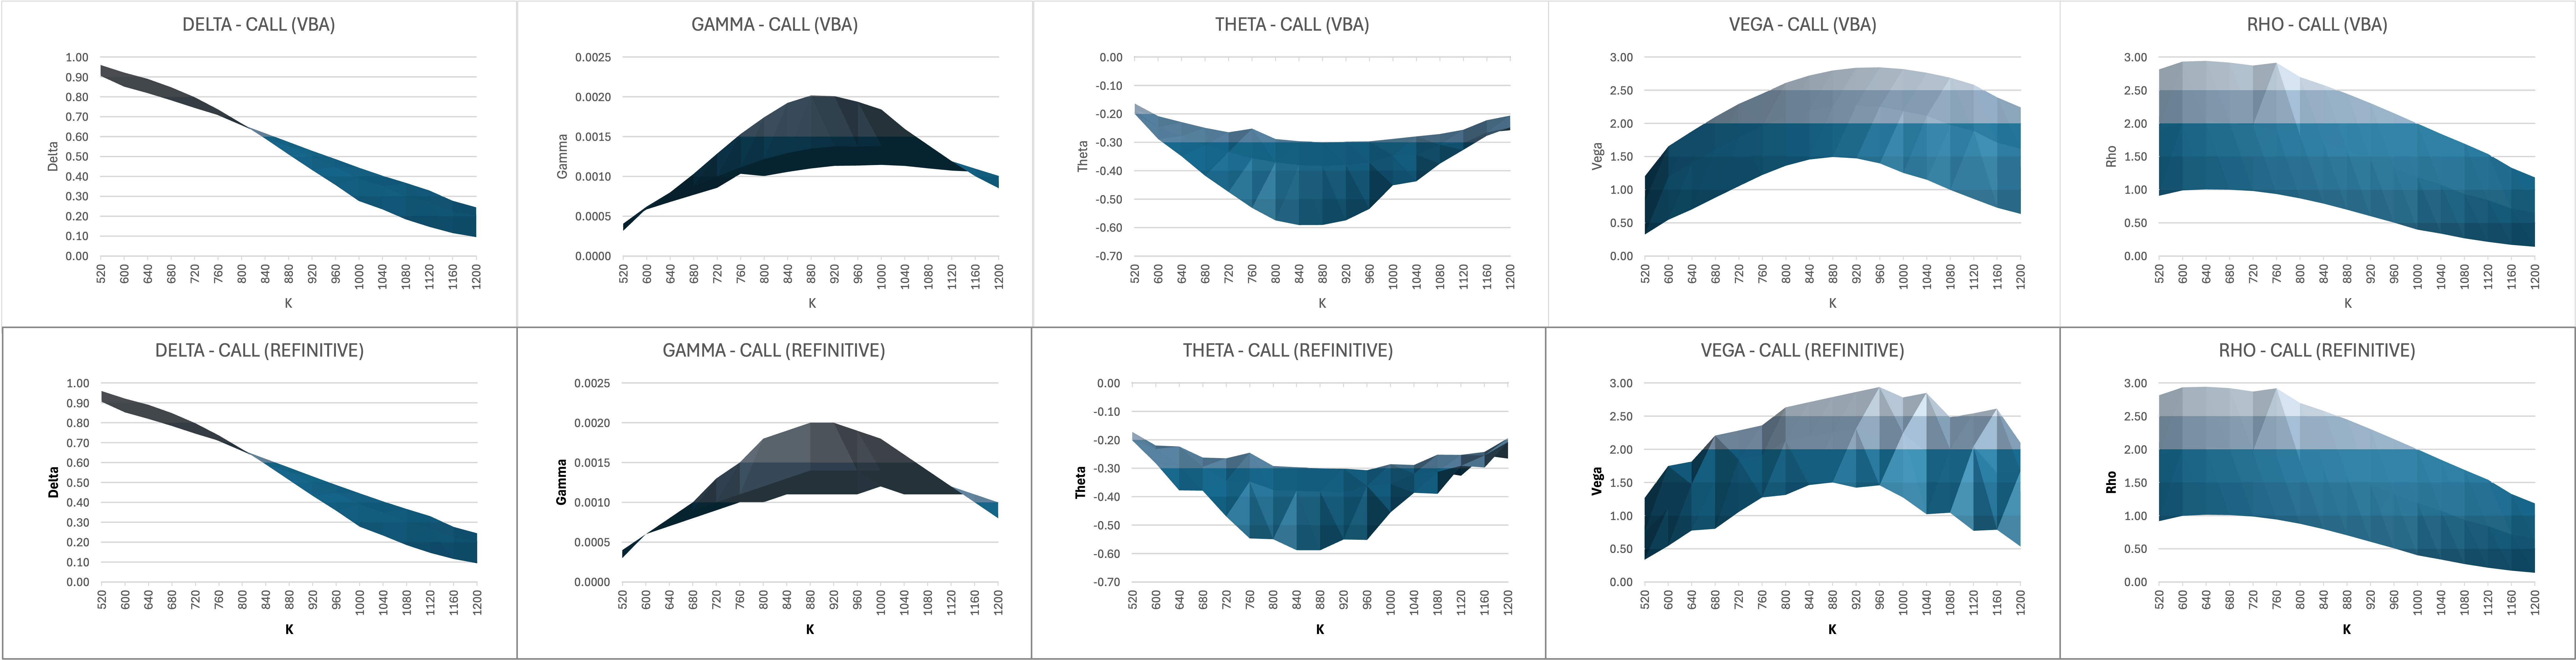
\includegraphics[width=\textwidth]{Picture5.png}
    \caption{3D Surfaces Comparison: VBA Model (top) vs Empirical Refinitiv Data (bottom). The horizontal axis is the Strike Price ($K$), representing a static cross-section of the option chain. The VBA surfaces are mathematically smooth, while the empirical ones capture the pricing noise inherent in the actual market.}
    \label{fig:part3_comparison}
\end{figure}
 
In conclusion, the overlap of the surfaces confirms the consistency of the VBA code
with Refinitiv's market Greeks, with differences that can be explained by calculation
conventions rather than methodological errors. Using implied volatility as a dynamic input makes
the B\&S model an excellent pricing tool even in the presence of a market skew,
provided the formulas are fed with the correct IV mapping for each pair $(K,\tau)$.

\end{document}